\section{PaWS}

The introduction page presents overall information about PaWS and PIPS in the panel on the left side, as it is shown in the Figure \ref{fig:intro_page}.

\begin{figure}[h!]
  \centering
  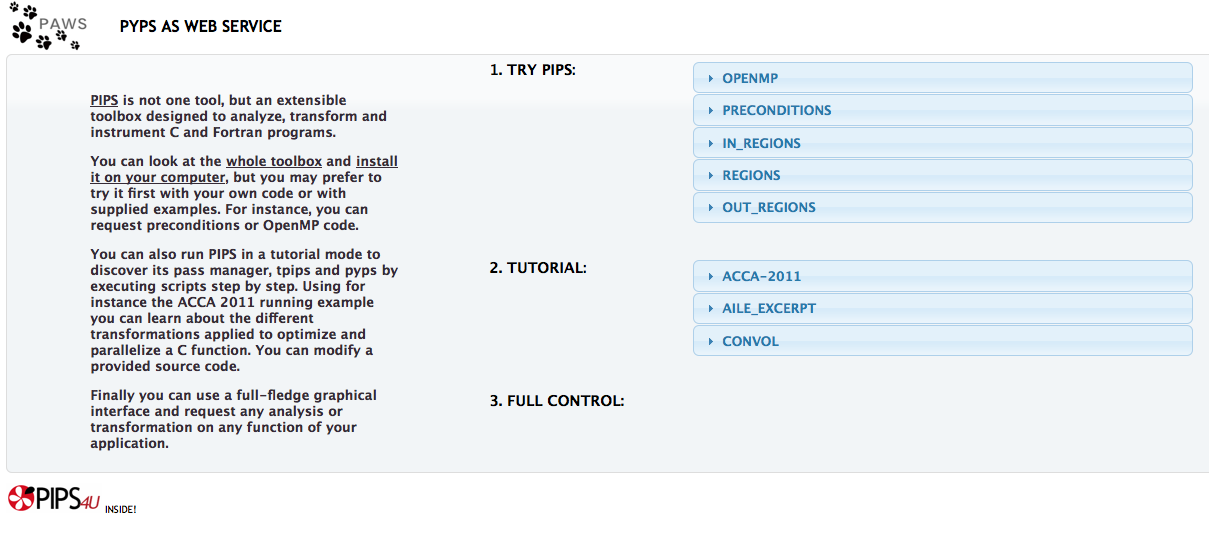
\includegraphics[width=0.8\textwidth]{reportCh4/intro_page}
  \caption{PaWS Introduction page.}
  \label{fig:intro_page}
\end{figure}

Left side panel allows the user to choose mode and its concrete tool or demonstration. To do it, the user has to click on the tab of the chosen tool/demonstration. It will be expanded (see Figure \ref{fig:expanded_tab}) with more detailed information and links to the actual sites visible.

\begin{figure}[h!]
  \centering
  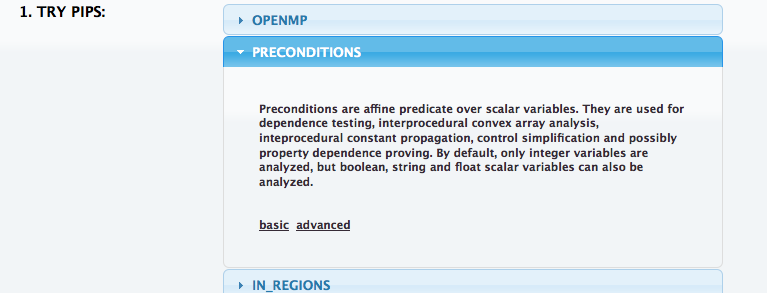
\includegraphics[width=1.0\textwidth]{reportCh4/expanded_tab}
  \caption{Expanded preconditions tab.}
  \label{fig:expanded_tab}
\end{figure}

To come back to the introduction page, the user can use logo image (see Figure \ref{fig:logo_image}) as a link.

\begin{figure}[h!]
  \centering
  
\includegraphics[width=0.2\textwidth]{reportCh4/logo_image}
  \caption{Logo image as home page link.}
  \label{fig:logo_image}
\end{figure}